% LaTeX .tex example for the proceedings of
% COBEM 2015 - 23rd International Congress of Mechanical Engineering
% November, 6-11 2015 - Rio de Janeiro, RJ, Brazil
%
% Based on the template of the proceedings of COBEM2013 

\documentclass[10pt,fleqn,a4paper,twoside]{article}
\usepackage{cobem2015}
\def\shortauthor{F. Author, S. Author and T. Author (update this heading accordingly)}
\def\shorttitle{Paper Short Title (First Letters Uppercase, make sure it fits in one line)}

\begin{document}
\fphead
\hspace*{-2.5mm}\begin{tabular}{||p{\textwidth}}
\begin{center}
\vspace{-4mm}
\title{INSTRUCTIONS FOR FORMATTING THE PROCEEDINGS PAPERS OF THE XXIII COBEM}
\end{center}
\authors{First Author's Name} \\
\authors{Second Author's Name} \\
\institution{Institution and address for first and second authors - if the same} \\
\institution{e-mails} \\
\\
\authors{Third Author's Name} \\
\institution{Institution and address for third author} \\
\institution{e-mail} \\
\\
\authors{Same format for others authors, if any} \\
\\
\abstract{\textbf{Abstract.} The purpose of these instructions is to serve as a guide for formatting papers to be published in the Proceedings of the XXIII COBEM. The abstract should describe the objectives, the methodology and the main conclusions of the paper in about 200 words. It should not contain neither formulae nor reference to bibliography. The abstract will be included in a printed volume to be distributed to the symposium participants, whilst the full paper will be published in the proceedings}\\
\\
\keywords{\textbf{Keywords:} keyword 1, keyword 2, keyword 3\dots{} (up to 5 keywords)}\\
\end{tabular}

\section{INTRODUCTION}

The proceedings of the XXIII COBEM will be published in Adobe\texttrademark\space PDF format.

The papers must be formatted strictly according to these instructions. The present file can be used as a template for \LaTeX\space users. Also, it should be used as a formatting guide to users of other text processing software.

The papers are limited to a maximum of 8 pages, including tables and figures. The final PDF file must not exceed 5.0 Mb.

\section{TEXT FORMAT}

The manuscripts should be written in English, typed in A4 size pages, using font Times New Roman, size 10, except for the title, authors affiliation, abstract and keywords, for which particular formatting instructions are indicated above. Single space between lines is to be used throughout the text.

The text block that contains the title, the authors' names and affiliation, the abstract and the keywords must be indented 0.1 cm from the left margin and marked by a leftmost black line border of width 2 1/4 pt.

The first page must have a top margin of 3 cm and all the other margins (left, right and bottom) must have 2 cm. All the other pages must be set with all margins equal to 2 cmf.

PAGES {\bf SHOULD NOT} BE NUMBERED

The body of the text must be justified. The first line of each paragraph must be indented by 0.5 cm. Sufficient information must be provided directly in the text, or by reference to widely available published work. Footnotes should be avoided.

All the symbols and notation must be defined in the text. Physical quantities must be expressed in the SI (metric) units. Mathematical symbols appearing in the text must be typed in italic style.

Bibliographic references should be cited in the text by giving the last name of the author(s) and the year of publication, according to the following examples: ``In a recent work~\citep{Vajjha:2009}\dots'' or ``Recently, \citet{Vajjha:2009}\dots''. In the case of three or more authors, the form ``\citep{Panaras:2010}'' should be used. Two or more references having the same authors and publication year must be distinguished by appending ``a'', ``b'', etc., to the year of publication. For exemple: ``In papers ~
~\citep{Simonson:1999a} and \citep{Simonson:1999b}\dots''.

Acceptable references include journal articles~\citep{Ozisik:1974}, numbered papers, dissertations and theses~\citep{Charoensupaya:Phd,Aparecido:PhD}, published conference proceedings~\citep{Tuckerman:2011}, preprints from conferences, books~\citep{Mikhailov:1984} and submitted articles (if the journal is identified). 


References should be listed at the end of the paper according to instructions provided in Section 4.

\subsection{Section titles and subtitles}

The section titles and subtitles must be aligned at left, typed with Times New Roman, size 10, bold style font. They must be numbered using Arabic numerals separated by points. No more than 3 sublevels should be used. One single line must be included above and bellow each section title/subtitle.

\subsection{Mathematical equations}

The mathematical equations must be indented by 0.5 cm from the left margin. They must be typed using Times New Roman, italic, size 10 pt. font.\ Arabic numerals must be used as equation numbers, enclosed between parentheses, right-aligned, as shown in the examples below. Equations should be referred to either as ``Eq.~(\ref{eq1})'' in the middle of a phrase or as ``Equation~(\ref{eq1})'' in the beginning of a sentence. Matrix and vector quantities can be indicated either by brackets and braces, as in Eq.~(\ref{eq1}), or in bold style, as in Eq.~(\ref{eq2}). Symbols used in the equations must be defined immediately before or after their first appearance.

One single line must be included above and bellow each equation.

\begin{equation}
[M]\{\ddot{x}\}+[C]\{\dot{x}(t)\}+[K]\{x(t)\}={f(t)} 
\label{eq1}
\end{equation}

\begin{equation}
\mathbf{M\ddot{x}}(t)+\mathbf{C\dot{x}}(t)+\mathbf{Kx}(t)=\mathbf{f}(t) 
\label{eq2}
\end{equation}


\subsection{Figures and tables}

Figures and tables should be placed in the text as close as possible to the point they are first mentioned and must be numbered consecutively in arabic numerals. Figures must be referred to either as ``Fig.~\ref{fig1}'' in the middle of a phrase or as ``Figure~\ref{fig1}'' in the beginning of a sentence. The figures themselves as well as their captions must be centered in the breadth-wise direction. The captions of the figures should not be longer than 3 lines.

The legend for the data symbols as well as the labels for each curve should be included into the figure. Lettering should be large enough for ease reading. All units must be expressed in the S.I. (metric) system.

One blank line must be left before and after each figure.

\begin{figure}[h!]
\centering
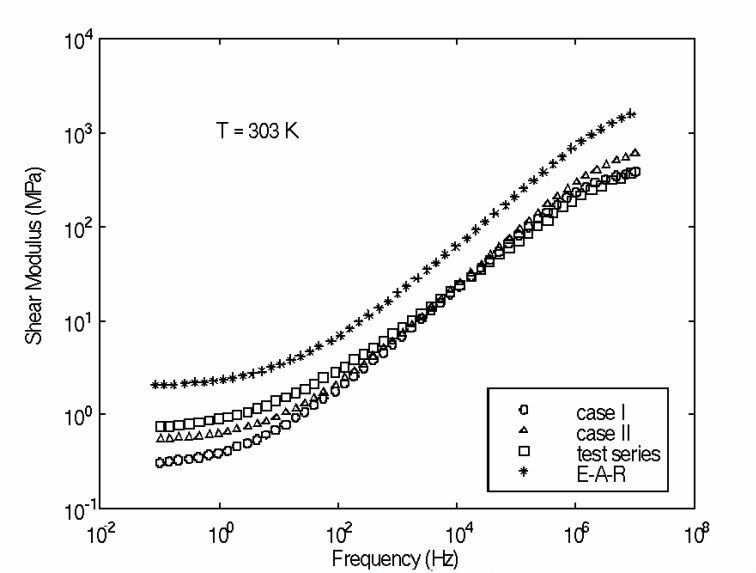
\includegraphics[angle=0, scale=1]{figure.jpg}
\caption{Diagram of shear modulus versus frequency at 303 K}
\label{fig1}
\end{figure}

Color figures and high quality photographs can be included in the paper. To reduce the file size and preserve the graphic resolution, figures must be saved into GIF (figures with less than 16 colors) or JPEG (for higher color density) files before being inserted in the manuscript.

Tables must be referred to either as ``Tab.~\ref{tab1}'' in the middle of a phrase or as ``Table~\ref{tab1}'' in the beginning of a sentence.  The tables themselves as well as their titles must be centered in the breadth-wise direction. The titles of the tables should not be longer than 3 lines. The font style and size used in the tables must be similar (both in size and style) to those used in the text body. Units must be expressed in the S.I.\ (metric) system. Explanations, if any, should be given at the foot of the tables, not within the tables themselves.

One blank line must be left before and after each table.

The style of table borders is left free. An example is given in Tab.~\ref{tab1}.

\begin{table}[!h]
\centering
\caption{Experimental results for flexural properties of CFRC-4HS and CFRC-TWILL composites. \protect\\Span/depth ratio = 35:1. Average results of 7 specimens.}
\begin{tabular}{|c|c|c|}
\hline
Composite Properties & CFRC-TWILL & CFRC-4HS\\
\hline
Flexural Strength (MPa)$^{(1)}$ & 209$\pm$ 10 & 180 $\pm$  15\\
\hline
Flexural Modulus (GPa)$^{(1)}$ & 57.0 $\pm$ 2.8 & 18.0 $\pm$  1.3\\
\hline
Mid-span deflection at the failure stress (mm) & 2.15 $\pm$  1.90 & 6.40 $\pm$  0.25\\
\hline
\end{tabular}
\\
\begin{tabular}{p{11cm}ll}
$^{(1)}$ measured at 25$^{o}$C & &
\end{tabular}
\label{tab1}
\end{table}

\section{ACKNOWLEDGEMENTS}
This optional section must be placed before the list of references.

\section{REFERENCES} 

The list of references must be introduced as a new section, located at the end of the paper. The first line of each reference must be aligned at left.  All the other lines must be indented by 0.5 cm from the left margin. All references included in the reference list must have been mentioned in the text.

References must be listed in alphabetical order, according to the last name of the first author. See the following examples:

\bibliographystyle{cobem2015}
\renewcommand{\refname}{}
\bibliography{bibfile}

\section{RESPONSIBILITY NOTICE}

The following text, properly adapted to the number of authors, must be included in the last section of the paper:

The author(s) is (are) the only responsible for the printed material included in this paper.

\end{document}
